\documentclass[12pt]{article} % Default font size is 12pt, it can be changed here
\usepackage{geometry} % Required to change the page size to A4
\geometry{a4paper} % Set the page size to be A4 as opposed to the default US Letter
\usepackage{graphicx} % Required for including pictures
\usepackage{float} % Allows putting an [H] in \begin{figure} to specify the exact location of the figure
\usepackage{wrapfig} % Allows in-line images such as the example fish picture
\linespread{1.2} % Line spacing
\graphicspath{{graphs/}} % Specifies the directory where pictures are stored
\usepackage{amssymb}

\begin{document}

%----------------------------------------------------------------------------------------
%	TITLE PAGE
%----------------------------------------------------------------------------------------
\begin{titlepage}

\newcommand{\HRule}{\rule{\linewidth}{0.5mm}} % Defines a new command for the horizontal lines, change thickness here

\center % Center everything on the page

\textsc{\LARGE Universit\'a di Trento}\\[0.8cm] % Name of your university/college
\textsc{\Large Corso HCI A.A. 2014-2015}\\[0.8cm] % Major heading such as course name
\textsc{\large Partecipatory Development}\\[1.5cm] % Minor heading such as course title

\HRule \\[0.8cm]
{ \huge \bfseries Gestione delle labels di Github}\\[0.4cm] % Title of your document
\HRule \\[2cm]

\begin{minipage}{0.4\textwidth}
\begin{flushleft} \large
\begin{tabular}{ll}
Bortoli \textsc{Gianluca} & \makebox[2cm][r]{159993} \\
Brugnara \textsc{Martin} & \makebox[2cm][r]{157791} \\
Dellera \textsc{Andrea} & \makebox[2cm][r]{158365} \\
Hoxha \textsc{Fatbardha} & \makebox[2cm][r]{161003}
\end{tabular}
\end{flushleft}
\end{minipage}

\vfill % Fill the rest of the page with whitespace
{\large \today}\\[3cm] % Date, change the \today to a set date if you want to be precise
\end{titlepage}

%----------------------------------------------------------------------------------------
%	TABLE OF CONTENTS
%----------------------------------------------------------------------------------------
\tableofcontents % Include a table of contents

\newpage % Begins the essay on a new page instead of on the same page as the table of contents 

\section{Introduzione}
Il primo obiettivo di questo progetto consiste nell'analizzare è quali siano le principali barriere nella partecipazione ai progetti open source, che oggigiorno sono diventati sempre più numerosi e di una certa rilevanza (addirittura a livello mondiale in alcuni casi).\\
Il nostro interesse è ricaduto proprio in queste problematiche che affliggono questo tipo di progetti, dal momento che sono state ravvisate anche in prima persona durante il corso dei nostri studi. \\
Questo approfondimento deriva in parte anche dalla nostra propensione ed interesse per l'utilizzo di software open source durante la nostra carriera universitaria e lavorativa.\\
Lo scopo finale è quello di trovare e formulare una possibile soluzione al problema della gestione delle etichette su Github (la piattaforma principe per lo sviluppo open source), dal momento che essa è attualmente molto confusionaria e poco ben gestita, soprattutto in progetti di una certa complessità e grandezza.
\newpage

\section{Interviste}
Il primo passo per l'individuazione delle principali problematiche legate all'ambito della partecipazione ai progetti open source è stata fatta tramite delle interviste. Questo tipo di ricerca si presta molto alla valutazione di barriere di questo tipo, dal momento che l'intervistato non si sente limitato nell'esprimersi (come potrebbe risultare da un questionario a risposta multipla), ma al contempo non ha la percezione di dilungarsi troppo (come invece potrebbe accadere se viene presentato un questionario a domanda aperta) che potrebbe indurlo a non scrivere tutto ciò che pensa. \\
Con il tramite dell'intervista "faccia a faccia" questi inconvenienti vengono meno: la persona si sente più libera di discutere con l'intervistatore che pone le domande e non blocca l'intervistato mentre sta rispondendo, non interrompendo così il flusso delle idee (che è la parte essenziale e di reale interesse dell'intera intervista).\\
\subsection{Traccia}
La traccia delle domande da porre all'intervistato ci è stata fornita direttamente dalla dottoressa Bordin, poiché tale argomento non era ancora stato trattato a lezione nel momento in cui abbiamo svolto questa parte del progetto.\\
Essa prevedeva delle domande mirate principalmente a capire:
\begin{itemize}
\item se e quali software open source vengono utilizzati
\item se l'intervistato partecipi/abbia partecipato attivamente a tali progetti
\item quali siano le motivazioni che lo hanno portato a farlo oppure no
\item cosa significhi \emph{partecipare} ad un progetto open source
%-----------------------------------------------------
% aggiungere link documento traccia bordin 
% http://disi.unitn.it/~deangeli/homepage/lib/exe/fetch.php?media=teaching:hci:hci2014_2015:intervista_pd_motivazioni.pdf
%-----------------------------------------------------
\end{itemize}
\subsection{Analisi dei risultati}
Il campione su cui è stata effettuata l'intervista non è molto eterogeneo (come è possibile vedere dalla Figura \ref{fig:distribuzione}), dal momento che è stato più immediato intervistare delle persone all'interno del nostro corso di laurea piuttosto che di altri atenei o dei lavoratori.

\begin{figure}[H] 
\center{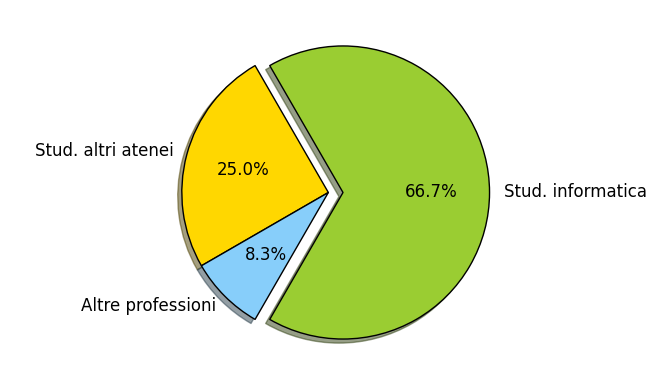
\includegraphics[width=0.8\linewidth]{interviewed_distribution.png}}
\caption{Distribuzione della professione delle persone intervistate.}
\label{fig:distribuzione}
\end{figure}

Abbiamo potuto notare come gli unici due intervistati che hanno contribuito attivamente a progetti open source provenissero esclusivamente da un ambito informatico. Inoltre, all'interno del gruppo stesso ben pochi lo hanno fatto, come è possibile notare dalla Figura \ref{fig:distribuzioneInformatica}.\\
Ciò ci permette di creare un profilo di utenza specifica (una \emph{personas}) in grado di prendere parte a questa tipologia di progetti. 

\begin{figure}[H] 
\center{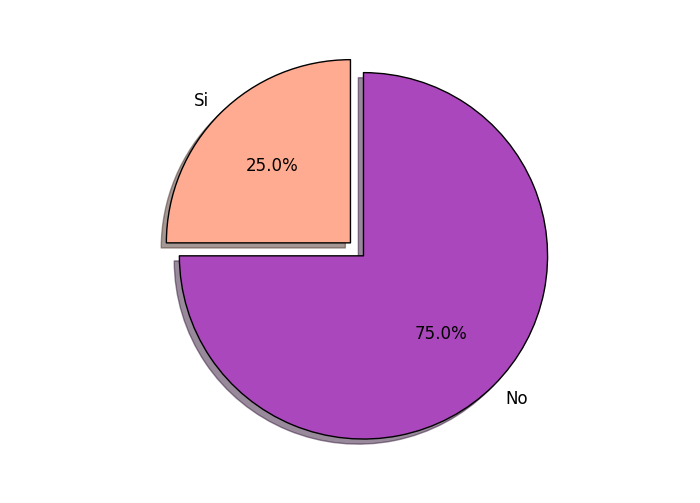
\includegraphics[width=0.8\linewidth]{interviewed_participation.png}}
\caption{Persone che hanno attivamente partecipato a progetti open source tra gli studenti di informatica.}
\label{fig:distribuzioneInformatica}
\end{figure}

Da ciò si evince che l'ambito e la possibilità di parteciparvi è molto ristretto e ciò ci permette di delineare una \emph{personas} con delle caratteristiche ben definite, quali:
\begin{itemize}
\item consistente background informatico
\item interesse verso il campo specifico del progetto considerato
\item tempo e impegno da dedicarvi
\end{itemize}

In aggiunta abbiamo notato come lo \emph{scenario} accademico incentivi e contribuisca ad utilizzare specifici software open source e, di conseguenza, aumenti la probabilità che uno studente si interessi e ne possa far parte. 
%-------
% descrizione di cosa sia una personas?
%-------
\newpage

\section{Benchmarking}
Durante questa fase abbiamo scelto di concentrarci su tre progetti open source in particolare: NeoVim, CyanogenMod e OpenOffice.\\
Dopo averli presentati e descritti durante un workshop, abbiamo analizzato i pro ed i contro di ciascuno, da cui in seguito abbiamo iniziato ad approfondire.\\
In primis, le motivazioni per contribuire ad un progetto open source sono molte: dalla semplice soddisfazione per aver risolto un bug, all'arricchimento personale e l'esperienza acquisita che ne conseguono, passando per la necessità di dover implementare una funzionalità che risolva un problema che si ha nel proprio lavoro.\\
Al contrario, altrettante sono i motivi che spingono le persone a non contribuire, tra i quali la mancanza di tempo e di competenze e soprattutto la qualità e disponibilità di informazioni riguardanti un progetto specifico. Quest'ultimo a nostro avviso risulta essere il più rilevante, dal momento che un utente (con magari delle capacità per farlo) si trova a non poter contribuire a causa della mancanza di linee guida su come si possa farlo. Ciò potrebbe sembrare banale a primo impatto, ma è una costante in tutti i progetti da noi presi in considerazione.
\newpage

\section{Design library}

\end{document}

%----------------
% miglioramenti: 
%				campione più eterogeneo e più vasto per le interviste
%---------------

